%%
%% This is file `sample-authordraft.tex',
%% generated with the docstrip utility.
%%
%% The original source files were:
%%
%% samples.dtx  (with options: `authordraft')
%% 
%% IMPORTANT NOTICE:
%% 
%% For the copyright see the source file.
%% 
%% Any modified versions of this file must be renamed
%% with new filenames distinct from sample-authordraft.tex.
%% 
%% For distribution of the original source see the terms
%% for copying and modification in the file samples.dtx.
%% 
%% This generated file may be distributed as long as the
%% original source files, as listed above, are part of the
%% same distribution. (The sources need not necessarily be
%% in the same archive or directory.)
%%
%% The first command in your LaTeX source must be the \documentclass command.
\documentclass[sigconf]{acmart}
%% NOTE that a single column version may be required for 
%% submission and peer review. This can be done by changing
%% the \doucmentclass[...]{acmart} in this template to 
%% \documentclass[manuscript,screen,review]{acmart}
%% 
%% To ensure 100% compatibility, please check the white list of
%% approved LaTeX packages to be used with the Master Article Template at
%% https://www.acm.org/publications/taps/whitelist-of-latex-packages 
%% before creating your document. The white list page provides 
%% information on how to submit additional LaTeX packages for 
%% review and adoption.
%% Fonts used in the template cannot be substituted; margin 
%% adjustments are not allowed.
%%
\usepackage{pgfplots}
\usepgfplotslibrary{fillbetween}
\usepackage{mathtools}
\newtheorem{resquest}{Research question}
\newtheorem*{resquest*}{Research question}

\usepackage[%
%    font={small,sf},
%    labelfont=bf,
%    format=hang,    
%    format=plain,
%    margin=0pt,
%    width=0.8\textwidth,
]{caption}
\usepackage[list=true]{subcaption}
\usepackage{color}
%
\definecolor{pblue}{rgb}{0.13,0.13,1}
\definecolor{pgreen}{rgb}{0,0.5,0}
\definecolor{pred}{rgb}{0.9,0,0}
\definecolor{pgrey}{rgb}{0.46,0.45,0.48}

\usepackage{listings}
\lstset{language=Java,
	showspaces=false,
	tabsize=2,
	frame=single,
	showtabs=false,
	breaklines=true,
	showstringspaces=false,
	breakatwhitespace=true,
	commentstyle=\color{pgreen},
	keywordstyle=\color{pblue},
	stringstyle=\color{pred},
	basicstyle=\ttfamily\scriptsize,
	moredelim=[il][\textcolor{pgrey}]{$$},
	moredelim=[is][\textcolor{pgrey}]{\%\%}{\%\%}
}

%% \BibTeX command to typeset BibTeX logo in the docs
\AtBeginDocument{%
  \providecommand\BibTeX{{%
    \normalfont B\kern-0.5em{\scshape i\kern-0.25em b}\kern-0.8em\TeX}}}

%% Rights management information.  This information is sent to you
%% when you complete the rights form.  These commands have SAMPLE
%% values in them; it is your responsibility as an author to replace
%% the commands and values with those provided to you when you
%% complete the rights form.
%\setcopyright{acmcopyright}
%\copyrightyear{2018}
%\acmYear{2018}
%\acmDOI{10.1145/1122445.1122456}

%% These commands are for a PROCEEDINGS abstract or paper.
%\acmConference[Woodstock '18]{Woodstock '18: ACM Symposium on Neural
%  Gaze Detection}{June 03--05, 2018}{Woodstock, NY}
%\acmBooktitle{Woodstock '18: ACM Symposium on Neural Gaze Detection,
%  June 03--05, 2018, Woodstock, NY}
%\acmPrice{15.00}
%\acmISBN{978-1-4503-XXXX-X/18/06}


%%
%% Submission ID.
%% Use this when submitting an article to a sponsored event. You'll
%% receive a unique submission ID from the organizers
%% of the event, and this ID should be used as the parameter to this command.
%%\acmSubmissionID{123-A56-BU3}

%%
%% The majority of ACM publications use numbered citations and
%% references.  The command \citestyle{authoryear} switches to the
%% "author year" style.
%%
%% If you are preparing content for an event
%% sponsored by ACM SIGGRAPH, you must use the "author year" style of
%% citations and references.
%% Uncommenting
%% the next command will enable that style.
%%\citestyle{acmauthoryear}

%%
%% end of the preamble, start of the body of the document source.
\begin{document}

%%
%% The "title" command has an optional parameter,
%% allowing the author to define a "short title" to be used in page headers.
\title{Something with Naturalize}

%%
%% The "author" command and its associated commands are used to define
%% the authors and their affiliations.
%% Of note is the shared affiliation of the first two authors, and the
%% "authornote" and "authornotemark" commands
%% used to denote shared contribution to the research.
\author{Noah Zuch}
\affiliation{%
  \institution{University of Passau}
  \department{Faculty of Computer Science and Mathematics, Chair of Software Engineering II}
  \streetaddress{Innstr. 43}
  \city{Passau}
  \country{Germany}
  \postcode{94032}
}
\email{zuch01@ads.uni-passau.de}


%%
%% By default, the full list of authors will be used in the page
%% headers. Often, this list is too long, and will overlap
%% other information printed in the page headers. This command allows
%% the author to define a more concise list
%% of authors' names for this purpose.
\renewcommand{\shortauthors}{Zuch}

%%
%% The abstract is a short summary of the work to be presented in the
%% article.
\begin{abstract}
  Programming languages allow for many diverse ways of solving the same problem. Some ways are considered bad practice and some follow coding conventions, found by practical experience. It should be in the best interest of every developer to follow such coding conventions if possible.
  %This is made hard by the fact that many projects declare new conventions or ignore existing ones.
  An automatic way of informing the programmer, that some coding convention got overlook is a hot research topic and many different approaches are explored. One possible approach is realized in the Naturalize tool, which uses N-gram models to informs the user about two specific coding convention: Badly chosen identifier names and bad formatting. But this approach has a few problems this paper want's to investigate: 1. Naturalize uses a different smoothing technique than stated to be optimal for code-modelling by other researchers. 2. Naturalize may tend to rely strongly on the presence of type-names to infer identifier names. 3. The evaluation done in the paper associated with Naturalize contains some inconsistencies when compared to the explanation of how Naturalize works. Besides an in-depth look into these inconsistencies, the empirical results of this paper show that 1. the proposedly better smoothing technique performs worse than the original one in Naturalize and 2. when removing type names Naturalize struggles to achieve acceptable results.
\end{abstract}

%%
%% The code below is generated by the tool at http://dl.acm.org/ccs.cfm.
%% Please copy and paste the code instead of the example below.
%%


%%
%% Keywords. The author(s) should pick words that accurately describe
%% the work being presented. Separate the keywords with commas.
\keywords{datasets, neural networks, gaze detection, text tagging}

%% A "teaser" image appears between the author and affiliation
%% information and the body of the document, and typically spans the
%% page.
%\begin{teaserfigure}
%  \includegraphics[width=\textwidth]{sampleteaser}
%  \caption{Seattle Mariners at Spring Training, 2010.}
%  \Description{Enjoying the baseball game from the third-base
%  seats. Ichiro Suzuki preparing to bat.}
%  \label{fig:teaser}
%\end{teaserfigure}

%%
%% This command processes the author and affiliation and title
%% information and builds the first part of the formatted document.
\maketitle

\section{Introduction}
% 1: Programing series of choices
% how to decompose problem into subproblems and fine grained how to name identifiers
% Naming improves the readability and cleanness of the code. This increases the maintainability ( 80% of time)
To program is to subdivide a complex problem hierarchically into smaller ones until at each level the problem is easily solvable. This ranges from dividing a program into micro-services to splitting up a complex method into multiple easier-to-understand parts.
%At every step of this subdivision the developer has think about how exactly the problem can be split up optimally.
An important goal is to make these subdivisions clear and understandable for future developers. Here a key principle is the explanatory naming of identifiers. This improves the readability and cleanness of the code and makes a program more maintainable. But correctly naming a given identifier be it a variable, a method, or a class is made difficult, because each development team and project has its own, maybe undocumented, rules for naming. To tackle this problem Allamins et al.~\cite{naturalize} introduced Naturalize, a tool that can learn naming and formatting conventions from a given source set and suggest names / formatting to the developer which are in line with the rest of the project. Internally Naturalize uses N-gram models to obtain an understanding of when which identifier name should be used. Eventthough Naturalize acchieves an accuracy of 94\% in its top suggestions for identifier names, there are a few areas where further research is required.

First, Naturalize uses Katz smoothing~\cite{naturalize} for its N-gram model, but without any explanation as to why. In another work, Hellendorn et al.~\cite{nestedngram} used nested N-grams together with deep learning to build a fast responding and nested modeling kit for programming languages. Their evaluations indicate that \texttt{JM} smoothing is the superior smoothing technique for modelling source code. Unfortunately Katz Smoohting was not part of their evaluation. This paper therefore tries to answer the following research question:

\begin{resquest}[RQ~\ref{hyp:jmsmoothing}] \label{hyp:jmsmoothing}
Does the usage of J-M Smoothing instead of Katz-Smoothing improve the accuracy of Naturalize?
\end{resquest}

Second, Naturalizes suggestions may be strongly biased. From manual investigation one can see, that for local variables, parameters, or fields Naturalize tends to rank the type-name of the variable (in lowercases) the highest. The same can be seen for methods, where Naturalize often suggest simple getter method names. A probable cause of this may be the close proximity of the variable name and type name in the java language, which enables the N-gram model to connect the to-be suggested identifier with other identifiers of the same type. Though this behaviour may be beneficial in some situations, an identifier name should probably convey more information than only its type. Like for which purpose a variable is created. Formed as a research questions this paper aims to answer:

\begin{resquest}[RQ~\ref{hyp:typeommitance}] \label{hyp:typeommitance}
How much impact does the type information in the code have on the suggestion accuracy of Naturalize?
\end{resquest}

Finally this paper discusses some significant inconsistencies between the evaluation described by Allamanis et al.~\cite{naturalize} and the associated source code on GitHub. More specifically this inconsitency lies in the fact that the explained evaluation strategy is simply not supported by the design of Naturalize. Probably of this reason a different approach is implemented in the source code.

\subsection{Contributions}
\begin{itemize}
    \item Investigating if Naturalize relies heavily on the existence of type names in the source code
    \item Modifying Naturalize to use JM Smoothing, which may improve accuracy
    \item Uncovering some inconsistencies in the evaluation of Naturalize
\end{itemize}

\section{Background}
This section summarizes the previous work of Allamanis et al.~\cite{naturalize} on the tool Naturalize and also gives an introduction to N-gram smoothing.
\subsection{Naturalize}
The goal of Naturalize was to automatically infer coding conventions out of some given source code
and then give suggestions to the programmer to better adhere to the found conventions.
They limited their scope to the naming of identifiers and code formatting. 
As this paper focuses on the naming part, the code formatting is excluded in this summary. 
The central concept of Naturalize is to use the well-known N-gram model to learn naming conventions from a given source set. Later this model can be used to suggest better alternative names for identifiers, which are more in line with the trained model. 
\begin{figure}
    \centering
    \graphicspath{{resources/}}  
    \def\svgwidth{0.5\textwidth}
    %% Creator: Inkscape 1.0.2 (e86c870879, 2021-01-15), www.inkscape.org
%% PDF/EPS/PS + LaTeX output extension by Johan Engelen, 2010
%% Accompanies image file 'naturalize_workflow.pdf' (pdf, eps, ps)
%%
%% To include the image in your LaTeX document, write
%%   \input{<filename>.pdf_tex}
%%  instead of
%%   \includegraphics{<filename>.pdf}
%% To scale the image, write
%%   \def\svgwidth{<desired width>}
%%   \input{<filename>.pdf_tex}
%%  instead of
%%   \includegraphics[width=<desired width>]{<filename>.pdf}
%%
%% Images with a different path to the parent latex file can
%% be accessed with the `import' package (which may need to be
%% installed) using
%%   \usepackage{import}
%% in the preamble, and then including the image with
%%   \import{<path to file>}{<filename>.pdf_tex}
%% Alternatively, one can specify
%%   \graphicspath{{<path to file>/}}
%% 
%% For more information, please see info/svg-inkscape on CTAN:
%%   http://tug.ctan.org/tex-archive/info/svg-inkscape
%%
\begingroup%
  \makeatletter%
  \providecommand\color[2][]{%
    \errmessage{(Inkscape) Color is used for the text in Inkscape, but the package 'color.sty' is not loaded}%
    \renewcommand\color[2][]{}%
  }%
  \providecommand\transparent[1]{%
    \errmessage{(Inkscape) Transparency is used (non-zero) for the text in Inkscape, but the package 'transparent.sty' is not loaded}%
    \renewcommand\transparent[1]{}%
  }%
  \providecommand\rotatebox[2]{#2}%
  \newcommand*\fsize{\dimexpr\f@size pt\relax}%
  \newcommand*\lineheight[1]{\fontsize{\fsize}{#1\fsize}\selectfont}%
  \ifx\svgwidth\undefined%
    \setlength{\unitlength}{406.04370117bp}%
    \ifx\svgscale\undefined%
      \relax%
    \else%
      \setlength{\unitlength}{\unitlength * \real{\svgscale}}%
    \fi%
  \else%
    \setlength{\unitlength}{\svgwidth}%
  \fi%
  \global\let\svgwidth\undefined%
  \global\let\svgscale\undefined%
  \makeatother%
  \begin{picture}(1,1.04562071)%
    \lineheight{1}%
    \setlength\tabcolsep{0pt}%
    \put(0,0){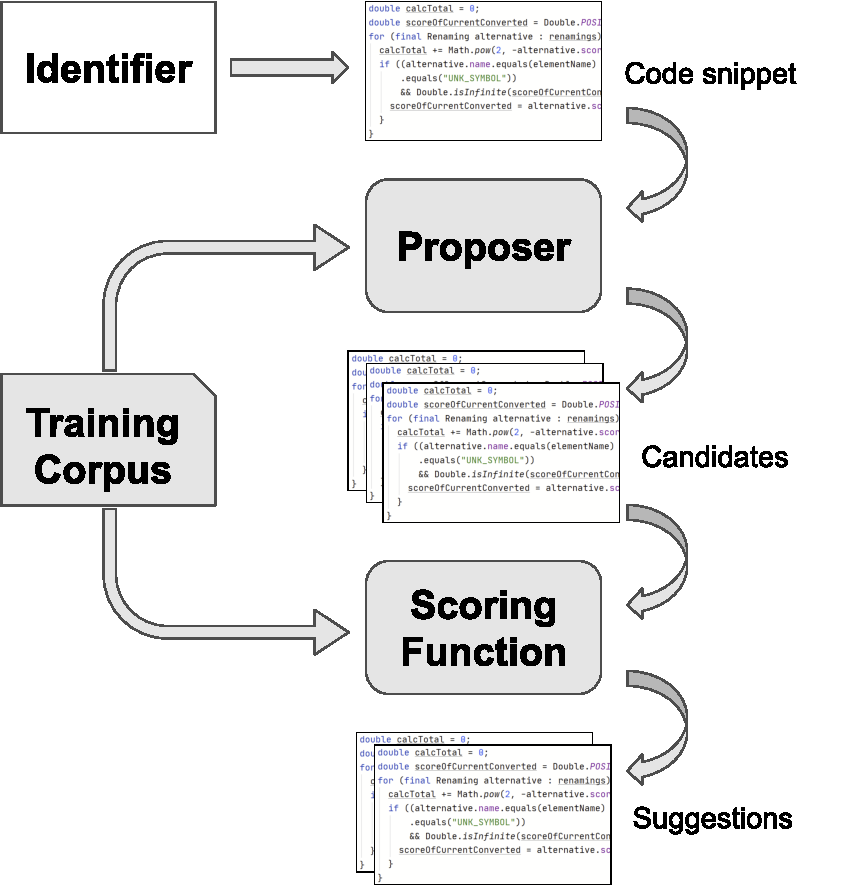
\includegraphics[width=\unitlength,page=1]{naturalize_workflow.pdf}}%
  \end{picture}%
\endgroup%

    \caption{Workflow of Naturalize}
    \label{fig:back_nat_workflow}
\end{figure}

In the learning phase, the tool converts a set of source files into token streams according to the
Java language definition and builds an N-gram model with them. Their findings indicate that a model of
order five is well suited.

After training Naturalize can now suggest alternative names for an identifier. The workflow for this task is shown in Figure~\ref{fig:back_nat_workflow}.
It starts with a request containing the identifier which should be renamed.
The intuitive idea behind Naturalize is that the name of an identifier depends on the code locations where the identifier is assigned or used. To be able to find those occurrences the initial request contains the AST node of the identifier in the Abstract Syntax Tree
of the current file. This allows Naturalize to find a parent node higher up in the tree, which encompasses all (local) occurrences of the identifier. An example: If the identifier is a local variable, the associated parent node is the AstNode representing the method, where the variable is defined. Then a code snippet is created, which simply contains the complete textual content of the parent node. This would, in the example above, be the signature and body of the defining method. It is important to mention that Naturalize, at least at the time this paper is being written,
does not include occurrences of identifiers outside of the current class. Now the N-gram model can be used to assign a probability to the code snippet indicating how in line this snippet, and therefore the identifier, is with the rest of the project.

Next, the Proposer has to find alternative names for the identifier. For this, the N-gram model is used. The code snippet is scanned and each N-gram, meaning each sub-snippet consisting of N words, which contains an occurrence of the identifier is extracted. Then the model is checked if it contains N-grams, which are similar to the extracted ones. Similar here means, that the N-gram only differs at the place, where the occurrence of the identifier is present. At this place the similar N-gram contains another identifier. These other identifiers are then used as the candidates for the suggestion. Corresponding code snippets for each candidate can be generated from the original one, by simply replacing the original name with the candidate name. As the last step, the scoring function ranks and filters the candidates. This is done by assigning a score to each candidate snippet using the N-gram model.
For filtering a threshold $t$ is introduced. This threshold controls which candidate should be filtered out by looking at their scores. Only those candidates with
a score greater than at least $t$ in comparison to the original name should be kept. The filtering also includes a parameter $k$, where only the top-$k$ suggestions are kept to not overburden the user with too many suggestions. The final list of suggestions is then presented to the user.

Some details which are not important for this paper were left out of this summary. For example how
Naturalize deals with unique rare names.

\subsection{N-gram smoothing}
Smoothing is an important part of language models that depend on N-grams. The basic equation for the estimated probability of a given N-gram $t=w_1^n=w_i\hdots w_n$ is
\begin{equation}
    P(w_n | w_1^{n-1}) =  \frac{C(w_1^n)}{C(w_1^{n-1})}
\end{equation}
where $C(w_1^n)$ is the number of times the sequence $w_1^n$ is present in the training set.
This simple equation, called the \emph{maximum likelihood} estimate, does not work well, as it assigns a zero score to N-grams that do not occur in the training set. These N-grams should obviously have a probability higher than zero. To solve this problem different smoothing methods can be applied~\cite{smoothingStudy}.

\subsubsection{Katz Smoothing}
Katz Smoothing is one of the simplest smoothing techniques. The basic idea is to use a lower order n-gram model (meaning a lower value of n) if the full n-gram occurs less than a given threshold $k$ times in the training set. This is repeated until a low enough n-gram model is found~\cite{katz1987estimation}. As an equation it can be written as:
\begin{equation}
    P(w_n | w_1^{n-1}) = 
    \begin{dcases}
    d_{w_1^{n-1}}\cdot \frac{C(w_1^n)}{C(w_1^{n-1})} & C(w_1^n) > k\\
    \alpha_{w_1^{n-1}} \cdot P(w_n | w_2^{n-1}) & \text{else}
    \end{dcases}
\end{equation}
The value $k$ is mostly, as also in Naturalize, chosen to be 1 and $d$ as well as $\alpha$ are pre-computed values per n-gram~\cite{katz1987estimation}.
\subsubsection{Jelinek and Mercer Smoothing}
Jelinek and Mercer Smoothing (JM Smoothing) also uses lower-order models to compute the final probability. But instead of using the first lower-order model with a high enough count, JM Smoothing interpolates over models of all orders~\cite{smoothingStudy}:
\begin{equation}
    P(w_n | w_1^{n-1})=\lambda_{w_1^{n-1}}\frac{C(w_1^n)}{C(w_1^{n-1})} + (1-\lambda_{w_1^{n-1}})P(w_n | w_2^{n-1})
\end{equation}
Again $\lambda_{w_1^{n-1}}$ are pre-trained values. Comparing these two methods the main difference between Katz and JM Smoothing is that Katz Smoothing stops at the first order, where the calculated probability is greater than zero, but JM continues to include lower-order models.

%\section{Methods}
%\subsection{Impact of Types}
From manual investigation one can see, that for local variables, parameters, or fields Naturalize tends to rank the type-name of the variable (in lowercases) the highest. A probable cause of this may be the close proximity of the variable name and type name in the java language, which enables the N-gram model to connect the to-be suggested identifier with other identifiers of the same type. 

\section{Evaluation}
The evaluation is build on top of the one done by Allamanis et al.~\cite{naturalize} in the original paper. At first, the test setup of the original authors is explained. Here the mentioned inconsistencies between the paper and the actual evaluation will be discussed. Then the results of a simple reevaluation of the test setup in the Github code will be presented. This reevaluation is to make sure, that my local setup results in the same values as in the original paper and also serves a baseline metric to answer the stated research questions. This baseline is especially important when considering the inconsistencies between the paper and the actual evaluation. Finally, the two research questions are answered.

\subsection{Methodology}
The corpus for evaluation is copied from the original paper. It is a set of well-known open-source java
projects selected by their number of "watchers" and forks. These projects combined with the used
commit hashes are presented in Table~\ref{tab:eval_projects}. The exact project \texttt{android-bootstrap} is no
longer available online but was superseded by another project. As it is hard to then find the correct commit, this project is left out.

The evaluation is done via a leave-one-out cross-validation on a per-project basis.
Meaning that, for each java file, Naturalize is trained on the other files in the current
project and evaluated on this single file. This is the recommended way of using Naturalize, as it excludes
the to-be-renamed identifiers from the training set. What exactly the rest of the files in each project means is a bit
ambiguous in the original paper. Some projects are divided into subprojects via Maven or Gradle. It is not clear whether these subprojects are evaluated separately or viewed as a single big project. This evaluation will train on all files, combining the subprojects into one. This approach should lead to better results as the model includes method names declared in one subproject and used in another.

\begin{table}
  \caption{Projects used for evaluation}
  \label{tab:eval_projects}
  \begin{tabular}{lr}
    \toprule
    Project&Commit\\
    \midrule
    elasticsearch&af17ae55\\
    libgdx&a42779e9\\
    netty&48eb73f9\\
    platform\_frameworks\_base&a0b320a6\\
    junit&d919bb6d\\
    wildfly&9d184cd0\\
    hudson&be1f8f91\\
    android-bootstrap&e2cde337\\
    k-9&d8030eaa\\
    android-menudrawer&96cdcdcc\\
    \bottomrule
\end{tabular}
\end{table}

\subsection{Rerunning the original evaluation}
To get a baseline for the other evaluations and to validate, that my setup results in the same values found
by the original authors, their evaluation is rerun. The focus here lies on the \emph{Single Point Suggestion},
where Naturalize is asked to find alternative names for a single identifier. Thankfully the authors provided
their code for the evaluation setup.

\subsubsection{Test-Setup in the Paper}
The explanation of their evaluation in the paper is as follows~\cite{naturalize}:
For each identifier in each file, Naturalize is asked to rename this identifier.
Here the suggestion accuracy is measured, meaning how often Naturalize suggests the original name in the top one
or top five suggestions. This assumes the original identifier to be correctly named.
The evaluation is redone for different values of the threshold $t$. A higher value of $t$ results in viewer
suggestions, as an alternative name has to have a much higher score than the original name, to not be
filtered out. This leads to having only suggestions of high accuracy but may permit Naturalize to give
any suggestions at all if no considerably better alternative is found. A low value of $t$ on the other hand results in
more suggestions of possibly worse accuracy.
The ratio of identifiers, where Naturalize is capable of finding an alternative, is called the suggestion frequency.
The results are then plotted into a 2d plot with suggestion frequency as the x-axis and suggestion accuracy as the y-axis. Such a plot is similar to a precision-recall curve, where values at the top right corner of the graph are better.

\subsubsection{Problem with the setup}
After looking in-depth into the evaluation logic provided on Github, it is clear that the setup above has a flaw. This claim is reinforced by the fact,
that the original authors used a different setup in their evaluation code as stated in
the paper. 

This difference is caused by the problem, that the evaluation expects the original name as a topmost candidate. Naturalize is not designed to support that. If the original name would be the top suggestion, every other suggestion would have been filtered out. Exactly in this case Naturalize is configured to not make a suggestion at all as no better alternative can be found. Which contradicts the expectation of having the original name as the top suggestion. But let's assume that an empty suggestion list is counted as if Naturalize would have suggested the original name. Then this results in Naturalize beeing able to always finding an alternative name and therefore the suggestion frequency has to be 100\% for any value of $t$. This is due to the fact that the frequency only drops in the above-mentioned case, where no \emph{other} alternative name is found. But this is now counted as if the original name is the suggestion. Now Naturalize can always suggest an alternative, sometimes another name other-times the original name. But the results of the original paper show, that they get suggestion frequencies below 100\% which contradicts the explanation of their setup.

This implies that they use a different setup than stated, and the setup in the source code actually differs. The actual setup is as follows:
For every renaming of an identifier the raw, unfiltered, suggestion list is returned and sorted by its score from lowest to highest. It is important to mention that the score is of log probability, so lower values are considered to be better. If the original name in the suggestion list has a score below or equal to the defined threshold $t$ it is counted as if Naturalize could give a suggestion. Notice that $t$ is now used as an absolute and not like designed as a relative threshold and it is applied to the original snippet and not to the other alternatives. Only if the original name passes this check, the accuracy gets evaluated. But this is also different from the paper. It is now checked, if the original name is under the top one / top five candidates of the unfiltered list, so without using the threshold $t$. In summary, the actual evaluation done in the source code differs substantially from the explanation in the paper. 

\subsubsection{Results}
\begin{figure*}
	\centering
	\subcaptionbox{Typenames}{%
	\begin{tikzpicture}[scale=0.65]
		\begin{axis}[xlabel = {Suggestion Frequency}, ylabel = {Suggestion Accuracy},
			axis x line =bottom, axis y line=left, ymin=0.7, ymax=1, xmin=0 , xmax=0.7, no markers, grid=major, ytick distance = {0.05}
		]
			\addplot [black, thick]coordinates {(0.1,1)		(0.18,0.99)		(0.23,0.96)		(0.27,0.95)		(0.3,0.94)		(0.33,0.94)		(0.35,0.94)		(0.38,0.93)		(0.44,0.92)		(0.49,0.91)		(0.55,0.88)		(0.6,0.85)		(0.73,0.78)		(0.79,0.73)		(0.82,0.72)		(0.82,0.72)		(0.82,0.72)		(0.82,0.72)		(0.82,0.72)	
};
			
			\addplot [name path=q1, gray] coordinates {(0.08,1)		(0.13,0.98)		(0.18,0.96)		(0.22,0.94)		(0.24,0.93)		(0.27,0.93)		(0.29,0.93)		(0.32,0.93)		(0.39,0.92)		(0.45,0.9)		(0.51,0.88)		(0.57,0.85)		(0.69,0.77)		(0.78,0.71)		(0.81,0.69)		(0.81,0.69)		(0.81,0.69)		(0.81,0.69)		(0.81,0.69)	

};
			
			\addplot [name path=q3, gray] coordinates {(0.09,1)		(0.19,1)		(0.26,0.98)		(0.31,0.97)		(0.34,0.96)		(0.36,0.96)		(0.39,0.96)		(0.42,0.96)		(0.48,0.95)		(0.53,0.94)		(0.58,0.92)		(0.63,0.9)		(0.75,0.84)		(0.81,0.79)		(0.84,0.77)		(0.84,0.77)		(0.84,0.77)		(0.84,0.77)		(0.84,0.77)	
	
};
			\tikzfillbetween[of=q1 and q3]{darkgray, opacity=0.4};
			
			
			\addplot [black, thick, dotted]coordinates {(0.1,1)		(0.18,1)		(0.23,0.99)		(0.27,0.98)		(0.3,0.97)		(0.33,0.97)		(0.35,0.97)		(0.38,0.96)		(0.44,0.95)		(0.49,0.94)		(0.55,0.92)		(0.6,0.9)		(0.73,0.85)		(0.79,0.81)		(0.82,0.8)		(0.82,0.8)		(0.82,0.8)		(0.82,0.8)		(0.82,0.8)	

};
			
			\addplot [name path=q15, gray] coordinates {(0.08,1)		(0.13,1)		(0.18,0.99)		(0.22,0.97)		(0.24,0.96)		(0.27,0.96)		(0.29,0.96)		(0.32,0.96)		(0.39,0.96)		(0.45,0.95)		(0.51,0.93)		(0.57,0.91)		(0.69,0.84)		(0.78,0.79)		(0.81,0.77)		(0.81,0.77)		(0.81,0.77)		(0.81,0.77)		(0.81,0.77)	

};
			
			\addplot [name path=q35, gray] coordinates {(0.09,1)		(0.19,1)		(0.26,1)		(0.31,0.99)		(0.34,0.99)		(0.36,0.99)		(0.39,0.99)		(0.42,0.99)		(0.48,0.98)		(0.53,0.97)		(0.58,0.96)		(0.63,0.95)		(0.75,0.89)		(0.81,0.86)		(0.84,0.84)		(0.84,0.84)		(0.84,0.84)		(0.84,0.84)		(0.84,0.84)	

};
			\tikzfillbetween[of=q15 and q35]{gray, opacity=0.4};
		\end{axis}
	\end{tikzpicture}
	}
	\subcaptionbox{Variables}{%
	\begin{tikzpicture}[scale=0.65]
		\begin{axis}[xlabel = {Suggestion Frequency}, ylabel = {Suggestion Accuracy},
			axis x line =bottom, axis y line=left, ymin=0.7, ymax=1, xmin=0 , xmax=0.7, no markers, grid=major, ytick distance = {0.05}
		]
		
		
			\addplot [black, thick]coordinates {(0.07,1)		(0.15,1)		(0.2,1)		(0.25,0.99)		(0.29,0.99)		(0.33,0.99)		(0.37,0.98)		(0.41,0.97)		(0.49,0.94)		(0.55,0.9)		(0.63,0.83)		(0.72,0.76)		(0.87,0.64)		(0.93,0.6)		(0.94,0.6)		(0.94,0.6)		(0.94,0.6)		(0.94,0.6)		(0.94,0.6)	

};
			
			\addplot [name path=q1, gray] coordinates {(0.06,1)		(0.11,1)		(0.16,0.99)		(0.2,0.99)		(0.25,0.99)		(0.29,0.98)		(0.34,0.97)		(0.38,0.96)		(0.47,0.93)		(0.53,0.88)		(0.59,0.8)		(0.67,0.7)		(0.88,0.6)		(0.94,0.57)		(0.95,0.57)		(0.95,0.57)		(0.95,0.57)		(0.95,0.57)		(0.95,0.57)	

};
			
			\addplot [name path=q3, gray] coordinates {(0.08,1)		(0.17,1)		(0.23,1)		(0.3,1)		(0.35,1)		(0.38,0.99)		(0.4,0.99)		(0.44,0.98)		(0.52,0.95)		(0.59,0.92)		(0.67,0.87)		(0.75,0.8)		(0.9,0.68)		(0.95,0.65)		(0.97,0.64)		(0.97,0.64)		(0.97,0.64)		(0.97,0.64)		(0.97,0.64)	

};
			\tikzfillbetween[of=q1 and q3]{darkgray, opacity=0.4};
			
			
			\addplot [black, thick, dotted]coordinates {(0.07,1)		(0.15,1)		(0.2,1)		(0.25,1)		(0.29,1)		(0.33,0.99)		(0.37,0.99)		(0.41,0.99)		(0.49,0.98)		(0.55,0.95)		(0.63,0.9)		(0.72,0.83)		(0.87,0.72)		(0.93,0.69)		(0.94,0.68)		(0.94,0.68)		(0.94,0.68)		(0.94,0.68)		(0.94,0.68)	


};
			
			\addplot [name path=q15, gray] coordinates {(0.06,1)		(0.11,1)		(0.16,1)		(0.2,1)		(0.25,1)		(0.29,0.99)		(0.34,0.99)		(0.38,0.99)		(0.47,0.97)		(0.53,0.94)		(0.59,0.88)		(0.67,0.8)		(0.88,0.7)		(0.94,0.67)		(0.95,0.66)		(0.95,0.66)		(0.95,0.66)		(0.95,0.66)		(0.95,0.66)	

};
			
			\addplot [name path=q35, gray] coordinates {(0.08,1)		(0.17,1)		(0.23,1)		(0.3,1)		(0.35,1)		(0.38,1)		(0.4,1)		(0.44,1)		(0.52,0.99)		(0.59,0.96)		(0.67,0.92)		(0.75,0.86)		(0.9,0.76)		(0.95,0.73)		(0.97,0.72)		(0.97,0.72)		(0.97,0.72)		(0.97,0.72)		(0.97,0.72)	


};
			\tikzfillbetween[of=q15 and q35]{gray, opacity=0.4};
		\end{axis}
	\end{tikzpicture}
	}
    \subcaptionbox{Method Calls}{%
	\begin{tikzpicture}[scale=0.65]
		\begin{axis}[xlabel = {Suggestion Frequency}, ylabel = {Suggestion Accuracy},
			axis x line =bottom, axis y line=left, ymin=0.7, ymax=1, xmin=0 , xmax=0.7, no markers, grid=major, ytick distance = {0.05}
		]
		
		
			\addplot [black, thick]coordinates {(0.11,1)		(0.21,0.97)		(0.29,0.94)		(0.34,0.92)		(0.38,0.91)		(0.41,0.89)		(0.45,0.87)		(0.48,0.85)		(0.55,0.8)		(0.62,0.76)		(0.68,0.72)		(0.74,0.68)		(0.82,0.63)		(0.86,0.61)		(0.87,0.6)		(0.87,0.6)		(0.87,0.6)		(0.87,0.6)		(0.87,0.6)	

};
			
			\addplot [name path=q1, gray] coordinates {(0.08,1)		(0.16,0.97)		(0.24,0.92)		(0.29,0.9)		(0.33,0.88)		(0.37,0.87)		(0.4,0.85)		(0.44,0.82)		(0.5,0.77)		(0.57,0.74)		(0.64,0.69)		(0.7,0.66)		(0.79,0.61)		(0.82,0.59)		(0.84,0.57)		(0.84,0.57)		(0.84,0.57)		(0.84,0.57)		(0.84,0.57)	


};
			
			\addplot [name path=q3, gray] coordinates {(0.12,1)		(0.25,0.98)		(0.35,0.96)		(0.4,0.94)		(0.44,0.92)		(0.46,0.91)		(0.5,0.89)		(0.54,0.87)		(0.59,0.84)		(0.66,0.8)		(0.72,0.76)		(0.78,0.72)		(0.87,0.67)		(0.9,0.65)		(0.91,0.63)		(0.91,0.63)		(0.91,0.63)		(0.91,0.63)		(0.91,0.63)	

};
			\tikzfillbetween[of=q1 and q3]{darkgray, opacity=0.4};
			
			
			\addplot [black, thick, dotted]coordinates {(0.11,1)		(0.21,1)		(0.29,0.99)		(0.34,0.98)		(0.38,0.97)		(0.41,0.96)		(0.45,0.95)		(0.48,0.94)		(0.55,0.9)		(0.62,0.86)		(0.68,0.83)		(0.74,0.8)		(0.82,0.76)		(0.86,0.74)		(0.87,0.73)		(0.87,0.73)		(0.87,0.73)		(0.87,0.73)		(0.87,0.73)	


};
			
			\addplot [name path=q15, gray] coordinates {(0.08,1)		(0.16,1)		(0.24,0.98)		(0.29,0.98)		(0.33,0.97)		(0.37,0.96)		(0.4,0.94)		(0.44,0.93)		(0.5,0.88)		(0.57,0.85)		(0.64,0.8)		(0.7,0.77)		(0.79,0.73)		(0.82,0.72)		(0.84,0.69)		(0.84,0.69)		(0.84,0.69)		(0.84,0.69)		(0.84,0.69)	

};
			
			\addplot [name path=q35, gray] coordinates {(0.12,1)		(0.25,1)		(0.35,0.99)		(0.4,0.98)		(0.44,0.98)		(0.46,0.97)		(0.5,0.96)		(0.54,0.95)		(0.59,0.92)		(0.66,0.89)		(0.72,0.86)		(0.78,0.83)		(0.87,0.79)		(0.9,0.77)		(0.91,0.77)		(0.91,0.77)		(0.91,0.77)		(0.91,0.77)		(0.91,0.77)	

};
			\tikzfillbetween[of=q15 and q35]{gray, opacity=0.4};
		\end{axis}
	\end{tikzpicture}
	}
	\caption{The results from the reevaluation of Naturalizes single point suggestion}
	\label{fig:eval_reeval_fig}
\end{figure*}
The result of the evaluation-rerun is presented in Figure~\ref{fig:eval_reeval_fig}.
As explained in the setup, each graph has on the y-axis the suggestion accuracy and on the x-axis the suggestion frequency. The result got split up into variables (meaning fields, parameters, and local variables), methods, and types (classes, enums, interfaces). Comparing the graphs with the ones in the original paper, one can see that the rerun produced roughly the same values indicating that the testing setup for the reevaluation is the same as the one originally used. 

\subsection{Impact of type names (RQ~\ref{hyp:typeommitance})}
This research question is concerned with the possibility that Naturalize relies heavily on the presence of type names in the code to give suggestions and is less suited to deduce identifier names from a more complex context.
\begin{figure*}
	\centering
%	\subcaptionbox{Typenames}{%
%	\begin{tikzpicture}[scale=0.65]
%		\begin{axis}[xlabel = {Suggestion Frequency},
%			axis x line =bottom, axis y line=left, ymin=0.7, ymax=1, xmin=0 , xmax=0.2, no markers, grid=major, ytick distance = {0.05}
%		]
%			\addplot [black, thick]coordinates {(0,1)		(0.01,1)		(0.01,0.98)		(0.02,0.96)		(0.02,0.96)		(0.02,0.95)		(0.03,0.92)		(0.03,0.87)		(0.04,0.82)		(0.05,0.79)		(0.06,0.77)		(0.07,0.76)		(0.09,0.68)		(0.11,0.59)		(0.12,0.55)		(0.12,0.55)		(0.12,0.55)		(0.12,0.55)		(0.12,0.55)	
%
%};
%			
%			\addplot [name path=q1, gray] coordinates {(0,1)		(0.01,1)		(0.01,0.96)		(0.02,0.97)		(0.02,0.96)		(0.02,0.96)		(0.02,0.96)		(0.03,0.89)		(0.04,0.86)		(0.04,0.83)		(0.05,0.8)		(0.06,0.77)		(0.08,0.68)		(0.1,0.58)		(0.1,0.54)		(0.11,0.54)	
%
%};
%			
%			\addplot [name path=q3, gray] coordinates {(0.01,1)			(0.02,1)		(0.02,0.99)		(0.03,0.99)		(0.03,0.99)		(0.03,0.98)		(0.04,0.95)		(0.04,0.89)		(0.05,0.86)		(0.06,0.85)		(0.07,0.85)		(0.09,0.77)		(0.11,0.66)		(0.12,0.62)		(0.12,0.61)	
%
%	
%};
%			\tikzfillbetween[of=q1 and q3]{darkgray, opacity=0.4};
%			
%			
%			\addplot [black, thick, dotted]coordinates {(0,1)		(0.01,1)		(0.01,0.99)		(0.02,0.99)		(0.02,0.98)		(0.02,0.98)		(0.03,0.95)		(0.03,0.9)		(0.04,0.87)		(0.05,0.85)		(0.06,0.83)		(0.07,0.82)		(0.09,0.76)		(0.11,0.69)		(0.12,0.66)		(0.12,0.66)		(0.12,0.66)		(0.12,0.66)		(0.12,0.66)	
%
%
%};
%			
%			\addplot [name path=q15, gray] coordinates {(0,1)		(0.01,1)		(0.01,0.99)		(0.02,0.99)		(0.02,0.99)		(0.02,0.99)		(0.02,0.98)		(0.03,0.91)		(0.04,0.89)		(0.04,0.87)		(0.05,0.86)		(0.06,0.86)		(0.08,0.77)		(0.1,0.69)		(0.1,0.67)		(0.11,0.66)	
%
%
%};
%			
%			\addplot [name path=q35, gray] coordinates {(0.01,1)			(0.02,1)		(0.02,0.99)		(0.03,1)		(0.03,0.99)		(0.03,0.99)		(0.04,0.97)		(0.04,0.94)		(0.05,0.92)		(0.06,0.9)		(0.07,0.89)		(0.09,0.82)		(0.11,0.75)		(0.12,0.73)		(0.12,0.71)	
%
%};
%			\tikzfillbetween[of=q15 and q35]{gray, opacity=0.4};
%		\end{axis}
%	\end{tikzpicture}
%	}
	\subcaptionbox{Variables}{%
	\begin{tikzpicture}[scale=0.65]
		\begin{axis}[xlabel = {Suggestion Frequency}, ylabel = {Suggestion Accuracy},
			axis x line =bottom, axis y line=left, ymin=0.7, ymax=1, xmin=0 , xmax=0.2, no markers, grid=major, ytick distance = {0.05}
		]
		
		
			\addplot [black, thick]coordinates {(0.01,1)		(0.01,1)		(0.02,0.99)		(0.02,0.99)		(0.03,0.98)		(0.03,0.98)		(0.04,0.97)		(0.04,0.95)		(0.05,0.91)		(0.06,0.84)		(0.07,0.74)		(0.09,0.61)		(0.13,0.44)		(0.14,0.4)		(0.15,0.39)		(0.15,0.39)		(0.15,0.39)		(0.15,0.39)		(0.15,0.39)	


};
			
			\addplot [name path=q1, gray] coordinates {(0,1)		(0.01,0.99)		(0.01,0.98)		(0.01,0.98)		(0.01,0.97)		(0.02,0.97)		(0.02,0.95)		(0.03,0.93)		(0.03,0.89)		(0.04,0.82)		(0.06,0.69)		(0.08,0.56)		(0.12,0.34)		(0.13,0.3)		(0.14,0.29)


};
			
			\addplot [name path=q3, gray] coordinates {(0.01,1)		(0.03,1)		(0.03,1)		(0.04,0.99)		(0.04,0.99)		(0.05,0.98)		(0.05,0.97)		(0.06,0.93)		(0.07,0.87)		(0.08,0.8)		(0.1,0.67)		(0.14,0.53)		(0.15,0.49)		(0.16,0.48)


};
		    \tikzfillbetween[of=q1 and q3]{darkgray, opacity=0.4};
			
			
			\addplot [black, thick, dotted]coordinates {(0.01,1)		(0.01,1)		(0.02,1)		(0.02,1)		(0.03,0.99)		(0.03,0.99)		(0.04,0.99)		(0.04,0.98)		(0.05,0.95)		(0.06,0.91)		(0.07,0.83)		(0.09,0.71)		(0.13,0.54)		(0.14,0.51)		(0.15,0.5)		(0.15,0.49)		(0.15,0.49)		(0.15,0.49)		(0.15,0.49)	



};
			
			\addplot [name path=q15, gray] coordinates {(0,1)		(0.01,1)		(0.01,0.99)		(0.02,0.98)		(0.02,0.98)		(0.03,0.97)		(0.03,0.94)		(0.04,0.88)		(0.06,0.79)		(0.08,0.65)		(0.12,0.48)		(0.13,0.45)		(0.14,0.44)	


};
			
			\addplot [name path=q35, gray] coordinates {(0.01,1)			(0.03,1)		(0.03,1)		(0.04,1)		(0.04,1)		(0.05,1)		(0.05,0.99)		(0.06,0.96)		(0.07,0.94)		(0.08,0.88)		(0.1,0.78)		(0.14,0.63)		(0.15,0.6)		(0.16,0.58)	



};
			\tikzfillbetween[of=q15 and q35]{gray, opacity=0.4};
		\end{axis}
	\end{tikzpicture}
	}
    \subcaptionbox{Method Calls}{%
	\begin{tikzpicture}[scale=0.65]
		\begin{axis}[xlabel = {Suggestion Frequency}, ylabel = {Suggestion Accuracy},
			axis x line =bottom, axis y line=left, ymin=0.7, ymax=1, xmin=0 , xmax=0.2, no markers, grid=major, ytick distance = {0.05}
		]
		
		
			\addplot [black, thick]coordinates {(0.01,1)		(0.03,0.97)		(0.05,0.89)		(0.07,0.82)		(0.09,0.77)		(0.1,0.74)		(0.11,0.69)		(0.12,0.67)		(0.14,0.63)		(0.15,0.58)		(0.17,0.54)		(0.18,0.51)		(0.19,0.48)		(0.2,0.47)		(0.2,0.46)		(0.2,0.46)		(0.2,0.46)		(0.2,0.46)		(0.2,0.46)	


};
			
			\addplot [name path=q1, gray] coordinates {(0.01,1)		(0.02,0.96)		(0.04,0.87)		(0.06,0.77)		(0.07,0.73)		(0.08,0.7)		(0.09,0.68)		(0.1,0.65)		(0.12,0.6)		(0.13,0.56)		(0.14,0.52)		(0.15,0.48)		(0.17,0.45)		(0.18,0.44)		(0.18,0.44)		(0.18,0.44)		(0.18,0.44)		(0.18,0.44)		(0.18,0.44)	



};
			
			\addplot [name path=q3, gray] coordinates {(0.01,1)		(0.03,0.99)		(0.07,0.93)		(0.09,0.83)		(0.11,0.77)		(0.12,0.74)		(0.13,0.71)		(0.14,0.7)		(0.15,0.66)		(0.17,0.61)		(0.19,0.58)		(0.21,0.55)		(0.22,0.52)		(0.22,0.5)		(0.22,0.5)		(0.22,0.5)		(0.22,0.5)		(0.22,0.5)		(0.22,0.5)	


};
			\tikzfillbetween[of=q1 and q3]{darkgray, opacity=0.4};
			
			
			\addplot [black, thick, dotted]coordinates {(0.01,1)		(0.03,1)		(0.05,0.97)		(0.07,0.92)		(0.09,0.89)		(0.1,0.86)		(0.11,0.83)		(0.12,0.81)		(0.14,0.77)		(0.15,0.72)		(0.17,0.68)		(0.18,0.65)		(0.19,0.61)		(0.2,0.59)		(0.2,0.59)		(0.2,0.59)		(0.2,0.59)		(0.2,0.59)		(0.2,0.59)	



};
			
			\addplot [name path=q15, gray] coordinates {(0.01,1)		(0.02,1)		(0.04,0.97)		(0.06,0.91)		(0.07,0.87)		(0.08,0.84)		(0.09,0.81)		(0.1,0.79)		(0.12,0.75)		(0.13,0.7)		(0.14,0.65)		(0.15,0.62)		(0.17,0.59)		(0.18,0.58)		(0.18,0.58)		(0.18,0.58)		(0.18,0.58)		(0.18,0.58)		(0.18,0.58)	


};
			
			\addplot [name path=q35, gray] coordinates {(0.01,1)		(0.03,1)		(0.07,0.99)		(0.09,0.93)		(0.11,0.89)		(0.12,0.88)		(0.13,0.84)		(0.14,0.82)		(0.15,0.79)		(0.17,0.76)		(0.19,0.71)		(0.21,0.68)		(0.22,0.63)		(0.22,0.62)		(0.22,0.62)		(0.22,0.62)		(0.22,0.62)		(0.22,0.62)		(0.22,0.62)	


};
			\tikzfillbetween[of=q15 and q35]{gray, opacity=0.4};
		\end{axis}
	\end{tikzpicture}
	}
	\caption{The results after obfuscating the type names.}
	\label{fig:eval_obfuscate_fig}
\end{figure*}
\subsubsection{Experimental Setup}
To answer this research question, Naturalize is modified to replace or remove concrete type names when reading the content of source files. More specifically type names are ignored/replaced in the training phase when creating a token stream and in the suggestion phase when creating the code snippet for suggestions. When rerunning the baseline evaluation with these modifications, n-gram model is forced to rely on contexts other than the type name.

\begin{figure}
    \centering
\begin{lstlisting}
%%@Override%%
public Multimap<Scope, String> getFromString(final String file,
		final ParseType parseType) {
	final Multimap<Scope, String> scopes = TreeMultimap.create();
	for (final IScopeExtractor extractor : allExtractors) {
		scopes.putAll(extractor.getFromString(file, parseType));
	}
	return scopes;
}
\end{lstlisting}%
\begin{lstlisting}
%%@Override%%
public getFromString(final var file,
		final var parseType) {
	final var scopes = TreeMultimap.create();
	for (final var extractor : allExtractors) {
		scopes.putAll(extractor.getFromString(file, parseType));
	}
	return scopes;
}
\end{lstlisting}%
    \caption{Sample Java code}
    \label{fig:meth_javacode}
\end{figure}

The idea is to change the Java-syntax of a source file in a way that it more mimics untyped languages. Figure~\ref{fig:meth_javacode} shows an example of an original and its modified java code. More precisely a source file/code snippet is modified in the following ways:

\begin{itemize}
    \item Variable/Field/Parameter declarations \texttt{<Type> <variableName>} get replaced with \texttt{var <variableName>}. This mimics in a sense the new Java 10 syntax.
    \item The Return type of methods get removed.
    \item All type arguments, e.g. generics, get removed.
    \item Object-Creation via \texttt{new <Type>(<parameters>)} stay as they are. There is no general rule to remove type information in an object's creation but still keep the semantics of the code. This is because object-oriented and strictly typed programming languages differ a great amount in the creation of structures to other languages.
    \item Other occurrences of Type-Names stay as they are. These include:
    \begin{itemize}
        \item Class/Interface/Enum-Declaration
        \item Types in qualified Names. E.g. \texttt{Stream.valueOf(...)}
        \item Class objects like \texttt{String.class}
    \end{itemize}
    These again can not be removed because such type names are still required to keep the semantics of the program.
\end{itemize}

To implement this modification of source code in Naturalize, I used the Abstract Syntax Tree functionality of the Eclipse JDT library~\cite{todo}. This library contains multiple classes which can print out source code for a given AST node. This class can then be modified to allow the above-mentioned modifications when printing out the code. In the training phase, Naturalize simply reads the content of each java file. Now an AST is created from each file and printed back as a String with the modifications. As a code-snippet for suggestion in Naturalize always consists of the content of exactly one AST node~\cite{naturalize}, this procedure can be directly adopted for code snippets.

\subsubsection{Results}
Figure~\ref{fig:eval_obfuscate_fig} shows the observed results when enabling the obfuscation of the type names in the code. For variable names explicitly the presumed behaviour was that removing type names from the source code significantly decreases the accuracy Naturalize can achieve. Looking at the results this assumption is confirmed as even for $k=5$ the accuracy already drops below 70\% at a frequency of only around 10\%. Comparing this with the results of the unobfuscated run, where the accuracy for $k=1$ does not drop below 70\% even for a frequency of over 70\%, a very big difference can be seen. For completeness also the results for type names and method names have been measured. A significant drop of the accuracy of type names is not unexpected, as exactly these type names got obfuscated. But also interestingly the accuracy for method names drops significantly compared to the normal evaluation. Here the accuracy drops below 70\% for $k=5$ at a frequency of only 16\%. This indicates that also the suggestion of method names relies strongly on type names. In this case probably on the return type and parameter type.
\noindent\fbox{\parbox{\linewidth}{%
\begin{resquest*}[RQ~\ref{hyp:typeommitance}]
How much impact does the type information in the code have on the suggestion accuracy of Naturalize?
\end{resquest*}
Naturalize relies heavily on the existence of type names to a point that removing only the type names from the source files produces a severely worse result.
}}


\subsection{J-M Smoothing (RQ~\ref{hyp:jmsmoothing})}
\begin{figure*}
	\centering
	\subcaptionbox{Typenames}{%
	\begin{tikzpicture}[scale=0.65]
		\begin{axis}[xlabel = {Suggestion Frequency}, ylabel = {Suggestion Accuracy},
			axis x line =bottom, axis y line=left, ymin=0.7, ymax=1, xmin=0 , xmax=0.7, no markers, grid=major, ytick distance = {0.05}
		]
			\addplot [black, thick]coordinates {(0.04,1)		(0.13,1)		(0.2,0.98)		(0.25,0.95)		(0.28,0.95)		(0.31,0.94)		(0.35,0.94)		(0.38,0.93)		(0.44,0.92)		(0.5,0.89)		(0.57,0.87)		(0.63,0.84)		(0.75,0.77)		(0.8,0.73)		(0.82,0.72)		(0.82,0.72)		(0.82,0.72)		(0.82,0.72)		(0.82,0.72)	


};
			
			\addplot [name path=q1, gray] coordinates {(0.03,1)		(0.1,1)		(0.16,0.98)		(0.2,0.95)		(0.23,0.94)		(0.26,0.94)		(0.3,0.94)		(0.33,0.93)		(0.4,0.92)		(0.48,0.9)		(0.54,0.87)		(0.6,0.83)		(0.72,0.75)		(0.79,0.7)		(0.8,0.69)		(0.81,0.69)		(0.81,0.69)		(0.81,0.69)		(0.81,0.69)	


};
			
			\addplot [name path=q3, gray] coordinates {(0.04,1)		(0.14,1)		(0.22,0.99)		(0.28,0.97)		(0.32,0.96)		(0.35,0.96)		(0.39,0.96)		(0.42,0.96)		(0.48,0.95)		(0.52,0.93)		(0.6,0.91)		(0.66,0.89)		(0.77,0.82)		(0.82,0.78)		(0.83,0.77)		(0.83,0.77)		(0.83,0.77)		(0.83,0.77)		(0.83,0.77)	


	
};
			\tikzfillbetween[of=q1 and q3]{darkgray, opacity=0.4};
			
			
			\addplot [black, thick, dotted]coordinates {(0.04,1)		(0.13,1)		(0.2,1)		(0.25,0.98)		(0.28,0.98)		(0.31,0.97)		(0.35,0.97)		(0.38,0.96)		(0.44,0.95)		(0.5,0.93)		(0.57,0.91)		(0.63,0.89)		(0.75,0.84)		(0.8,0.81)		(0.82,0.8)		(0.82,0.8)		(0.82,0.8)		(0.82,0.8)		(0.82,0.8)	



};
			
			\addplot [name path=q15, gray] coordinates {(0.03,1)		(0.1,1)		(0.16,1)		(0.2,0.98)		(0.23,0.97)		(0.26,0.96)		(0.3,0.96)		(0.33,0.96)		(0.4,0.95)		(0.48,0.94)		(0.54,0.92)		(0.6,0.89)		(0.72,0.82)		(0.79,0.78)		(0.8,0.77)		(0.81,0.77)		(0.81,0.77)		(0.81,0.77)		(0.81,0.77)	

};
			
			\addplot [name path=q35, gray] coordinates {(0.04,1)		(0.14,1)		(0.22,1)		(0.28,1)		(0.32,0.99)		(0.35,0.99)		(0.39,0.99)		(0.42,0.98)		(0.48,0.98)		(0.52,0.97)		(0.6,0.96)		(0.66,0.94)		(0.77,0.88)		(0.82,0.85)		(0.83,0.84)		(0.83,0.84)		(0.83,0.84)		(0.83,0.84)		(0.83,0.84)	

};
			\tikzfillbetween[of=q15 and q35]{gray, opacity=0.4};
		\end{axis}
	\end{tikzpicture}
	}
	\subcaptionbox{Variables}{%
	\begin{tikzpicture}[scale=0.65]
		\begin{axis}[xlabel = {Suggestion Frequency}, ylabel = {Suggestion Accuracy},
			axis x line =bottom, axis y line=left, ymin=0.7, ymax=1, xmin=0 , xmax=0.7, no markers, grid=major, ytick distance = {0.05}
		]
		
		
			\addplot [black, thick]coordinates {(0.03,1)		(0.1,1)		(0.17,1)		(0.23,0.99)		(0.27,0.99)		(0.32,0.99)		(0.36,0.98)		(0.41,0.97)		(0.49,0.94)		(0.57,0.88)		(0.66,0.8)		(0.76,0.72)		(0.9,0.62)		(0.93,0.6)		(0.93,0.6)		(0.93,0.6)		(0.93,0.6)		(0.93,0.6)		(0.93,0.6)	



};
			
			\addplot [name path=q1, gray] coordinates {(0.02,1)		(0.08,1)		(0.14,1)		(0.18,0.99)		(0.23,0.99)		(0.28,0.99)		(0.32,0.98)		(0.36,0.96)		(0.44,0.93)		(0.52,0.87)		(0.6,0.77)		(0.71,0.67)		(0.9,0.59)		(0.94,0.56)		(0.94,0.56)		(0.94,0.56)		(0.94,0.56)		(0.94,0.56)		(0.94,0.56)	

};
			
			\addplot [name path=q3, gray] coordinates {(0.03,1)		(0.11,1)		(0.2,1)		(0.27,1)		(0.32,1)		(0.36,0.99)		(0.4,0.99)		(0.44,0.98)		(0.53,0.95)		(0.61,0.9)		(0.7,0.84)		(0.8,0.76)		(0.92,0.65)		(0.96,0.63)		(0.96,0.63)		(0.96,0.63)		(0.96,0.63)		(0.96,0.63)		(0.96,0.63)	

};
		    \tikzfillbetween[of=q1 and q3]{darkgray, opacity=0.4};
			
			
			\addplot [black, thick, dotted]coordinates {(0.03,1)		(0.1,1)		(0.17,1)		(0.23,1)		(0.27,1)		(0.32,1)		(0.36,0.99)		(0.41,0.99)		(0.49,0.98)		(0.57,0.94)		(0.66,0.87)		(0.76,0.8)		(0.9,0.71)		(0.93,0.69)		(0.93,0.69)		(0.93,0.69)		(0.93,0.69)		(0.93,0.69)		(0.93,0.69)	



};
			
			\addplot [name path=q15, gray] coordinates {(0.02,1)		(0.08,1)		(0.14,1)		(0.18,1)		(0.23,1)		(0.28,1)		(0.32,0.99)		(0.36,0.99)		(0.44,0.97)		(0.52,0.93)		(0.6,0.85)		(0.71,0.77)		(0.9,0.69)		(0.94,0.67)		(0.94,0.67)		(0.94,0.67)		(0.94,0.67)		(0.94,0.67)		(0.94,0.67)	

};
			
			\addplot [name path=q35, gray] coordinates {(0.03,1)		(0.11,1)		(0.2,1)		(0.27,1)		(0.32,1)		(0.36,1)		(0.4,1)		(0.44,1)		(0.53,0.98)		(0.61,0.95)		(0.7,0.9)		(0.8,0.82)		(0.92,0.74)		(0.96,0.73)		(0.96,0.73)		(0.96,0.73)		(0.96,0.73)		(0.96,0.73)		(0.96,0.73)	


};
			\tikzfillbetween[of=q15 and q35]{gray, opacity=0.4};
		\end{axis}
	\end{tikzpicture}
	}
    \subcaptionbox{Method Calls}{%
	\begin{tikzpicture}[scale=0.65]
		\begin{axis}[xlabel = {Suggestion Frequency}, ylabel = {Suggestion Accuracy},
			axis x line =bottom, axis y line=left, ymin=0.7, ymax=1, xmin=0 , xmax=0.7, no markers, grid=major, ytick distance = {0.05}
		]
		
		
			\addplot [black, thick]coordinates {(0.03,1)		(0.14,0.99)		(0.22,0.96)		(0.3,0.93)		(0.35,0.91)		(0.39,0.9)		(0.43,0.87)		(0.47,0.85)		(0.55,0.79)		(0.62,0.74)		(0.69,0.7)		(0.75,0.66)		(0.83,0.61)		(0.85,0.59)		(0.86,0.59)		(0.86,0.59)		(0.86,0.59)		(0.86,0.59)		(0.86,0.59)	


};
			
			\addplot [name path=q1, gray] coordinates {(0.02,1)		(0.1,0.99)		(0.19,0.95)		(0.26,0.91)		(0.31,0.9)		(0.35,0.88)		(0.39,0.86)		(0.43,0.83)		(0.5,0.77)		(0.57,0.72)		(0.65,0.67)		(0.71,0.63)		(0.78,0.59)		(0.82,0.58)		(0.82,0.57)		(0.82,0.57)		(0.82,0.57)		(0.82,0.57)		(0.82,0.57)	


};
			
			\addplot [name path=q3, gray] coordinates {(0.04,1)		(0.16,1)		(0.26,0.97)		(0.33,0.95)		(0.38,0.93)		(0.42,0.91)		(0.46,0.88)		(0.5,0.85)		(0.58,0.8)		(0.66,0.76)		(0.74,0.72)		(0.8,0.68)		(0.87,0.64)		(0.89,0.61)		(0.9,0.61)		(0.9,0.61)		(0.9,0.61)		(0.9,0.61)		(0.9,0.61)	

};
			\tikzfillbetween[of=q1 and q3]{darkgray, opacity=0.4};
			
			
			\addplot [black, thick, dotted]coordinates {(0.03,1)		(0.14,1)		(0.22,1)		(0.3,0.98)		(0.35,0.98)		(0.39,0.97)		(0.43,0.96)		(0.47,0.94)		(0.55,0.89)		(0.62,0.85)		(0.69,0.82)		(0.75,0.79)		(0.83,0.75)		(0.85,0.74)		(0.86,0.74)		(0.86,0.74)		(0.86,0.74)		(0.86,0.74)		(0.86,0.74)	

};
			
			\addplot [name path=q15, gray] coordinates {(0.02,1)		(0.1,1)		(0.19,1)		(0.26,0.98)		(0.31,0.97)		(0.35,0.96)		(0.39,0.95)		(0.43,0.93)		(0.5,0.88)		(0.57,0.84)		(0.65,0.8)		(0.71,0.77)		(0.78,0.74)		(0.82,0.71)		(0.82,0.71)		(0.82,0.71)		(0.82,0.71)		(0.82,0.71)		(0.82,0.71)	

};
			
			\addplot [name path=q35, gray] coordinates {(0.04,1)		(0.16,1)		(0.26,1)		(0.33,0.99)		(0.38,0.98)		(0.42,0.97)		(0.46,0.96)		(0.5,0.94)		(0.58,0.91)		(0.66,0.87)		(0.74,0.84)		(0.8,0.81)		(0.87,0.77)		(0.89,0.77)		(0.9,0.77)		(0.9,0.77)		(0.9,0.77)		(0.9,0.77)		(0.9,0.77)	


};
			\tikzfillbetween[of=q15 and q35]{gray, opacity=0.4};
		\end{axis}
	\end{tikzpicture}
	}
	\caption{The results when  using J-M smoothing}
	\label{fig:eval_JM_fig}
\end{figure*}
The second research question was about which smoothing techniques, recommended by different researches, is best suited for the N-gram model in Naturalize. Specifically Katz Smoothing and JM Smoothing should be compared.

For JM smoothing the values $\lambda_{w_1^{n-1}}$ have to be precomputed. Hellendorn et al.~\cite{nestedngram} set these to always be $0.5$. So no matter which n-gram order, the maximum likelihood of the current order has the same weight as the result of the lower order model. Why these specific parameter values are used is not justified. Assuming that the configuration $\lambda_{w_1^{n-1}}=0.5$ was chosen for a reason this configuration is kept for the evaluation. Figure~\ref{fig:eval_JM_fig} presents the results when replacing Katz smoothing in Naturalize with the JM Smoothing approach. When comparing the graphs with the baseline in Figure~\ref{fig:eval_reeval_fig} no big difference can be observed. J-M Smoothing tends to have a smaller inner quartile range, indicating more consistent results over different projects. On the other side the average accuracy of Katz Smoothing tends to be slightly higher than J-M smoothing.
\noindent\fbox{\parbox{\linewidth}{%
\begin{resquest*}[RQ~\ref{hyp:jmsmoothing}]
Does the usage of JM Smoothing instead of Katz-Smoothing improve the accuracy of Naturalize?
\end{resquest*}
JM Smoothing does not produce a significantly better result in Naturalize than Katz Smoothing. It actually decreases the achieved accuracy by a slight amount.
}}

\section{Threats to validity}
\subsection{External Validity}
Threats to \emph{external validity} are concerned with the possibility, that the results of the evaluation can not be generalized outside of the testing setup scope. The main factor to reason about in this study is the selection of projects used for the evaluation. Allamanis et al.~\cite{naturalize} have already discussed this problem and came to the conclusion, that their careful selection of the testing projects ensures the generalizability of the results. This can also be directly applied to the evaluation made in this paper, as it uses the same test setup.

\subsection{Internal Validity}
Threats to \emph{internal validity} are concerned with the possibility that the relationship between treatment and outcome of an evaluation is not causal, but rather influenced by factors over which the evaluation has no control or does not concretely specify. Some small tweaks to the original source code of Naturalize were performed, which could potentially change the outcome of the tool. But these changes are only to make Naturalize more performant in the tests and do not change any logic. The result of the reevaluation supports this claim. The comparison between the results of the original study and the reevaluation supports this claim.
As the setup of the evaluation between the baseline and the modified version only differs in one specific change, no uncontrolled factors should exist. To make sure, that the evaluation is specified as concretely as possible, the source code of the modifications and evaluation is made publicly available under the following link: \href{A Link between Sites}{\url{https://de.wikipedia.org/wiki/The_Legend_of_Zelda:_A_Link_Between_Worlds}}.

\subsection{Conclusion Validity}
Threats to \emph{conclusion validity} limit the degree to which conclusions about the relationship between variables from the resulting data are correct or reasonable. Different from most other machine learning tools, N-gram models are a deterministic approach so the results can not be influenced by some random variable. Also, the results from the original study are used to bring the observed values into context.
\section{Discussion}
The results of the type name obfuscation are unexpectedly worse than the baseline. A drop in accuracy is expected as it makes sense, that a local N-gram model can use the type name of a variable to associate it with other variables of the same type. But a such severe drop indicates that Naturalize almost exclusively relies on the type names. This poses the concern,that Naturalize is not able to achieve even mildly acceptable results when applied to a dynamically typed language like JavaScript instead of Java.

The comparison between the smoothing techniques, at least in Naturalize, showed that JM Smoothing can not improve the accuracy when compared to Katz smoothing. In fact it slightly decreases it. JM Smoothing was found to be the superior smoothing technique by Hellendorn et al.~\cite{nestedngram} for their nested language model. As they did not include Katz Smoothing in their survey the question arises if Katz smoothing may not only be beneficial in Naturalize but also in the nested language model of Hellendorn et al.

This paper also uncovered some inconsistencies between the evaluation setup explained by Allamanis et al.~\cite{naturalize} and the actual evaluation code. These inconsistencies result from the fact that the evaluation as explained in the paper is not compatible with the designed functionality of Naturalize. A better evaluation setup may be to rename all occurences of the identifier for which alternative names should be found. This renaming also has to include occurrence outside of the current file and the new name should be something obviously unnatural. Now the accuracy can be measured meaning how often Naturalize would suggest the original name before the refacoring. And also the suggestion frequency can be measured correctly as now Naturalize may not be able to suggest alternatives for the renamed junk name. This is also a lot closer to reality as the usage of a class in the rest of the project may tend to bias the model to prefer the current name over an alternative.
\section{Related work}

\section{Summary}
This paper showed that JM Smoothing, recommended by other researchers, can not improve the accuracy of Naturalize when using it instead of the default Katz Smoothing technique. Also some problems with the Naturalize tool are discussed including an inconsistent evaluation and the concern that Naturalizes good results are only applicable to strictly typed programming languages. Machine learning enables tools for software engineering to be theoretically usable over a wide range of programming languages. But the syntax of each programming language may change the level of effectiveness of such a model. Claiming that a tool can be used over multiple languages should therefore be stated with care and preferably with prior evaluation. In the discussion section some possible implications are given, which would make good content for further research as there was not enough time to cover them in this paper.





%%% The next two lines define the bibliography style to be used, and
%%% the bibliography file.
\bibliographystyle{ACM-Reference-Format}
\bibliography{sample-base}

\end{document}
\endinput

